% !TEX root = main.tex

\chapter{Overview}
\label{ch:overview}
\noindent


\begin{figure}[t]
  \centerline{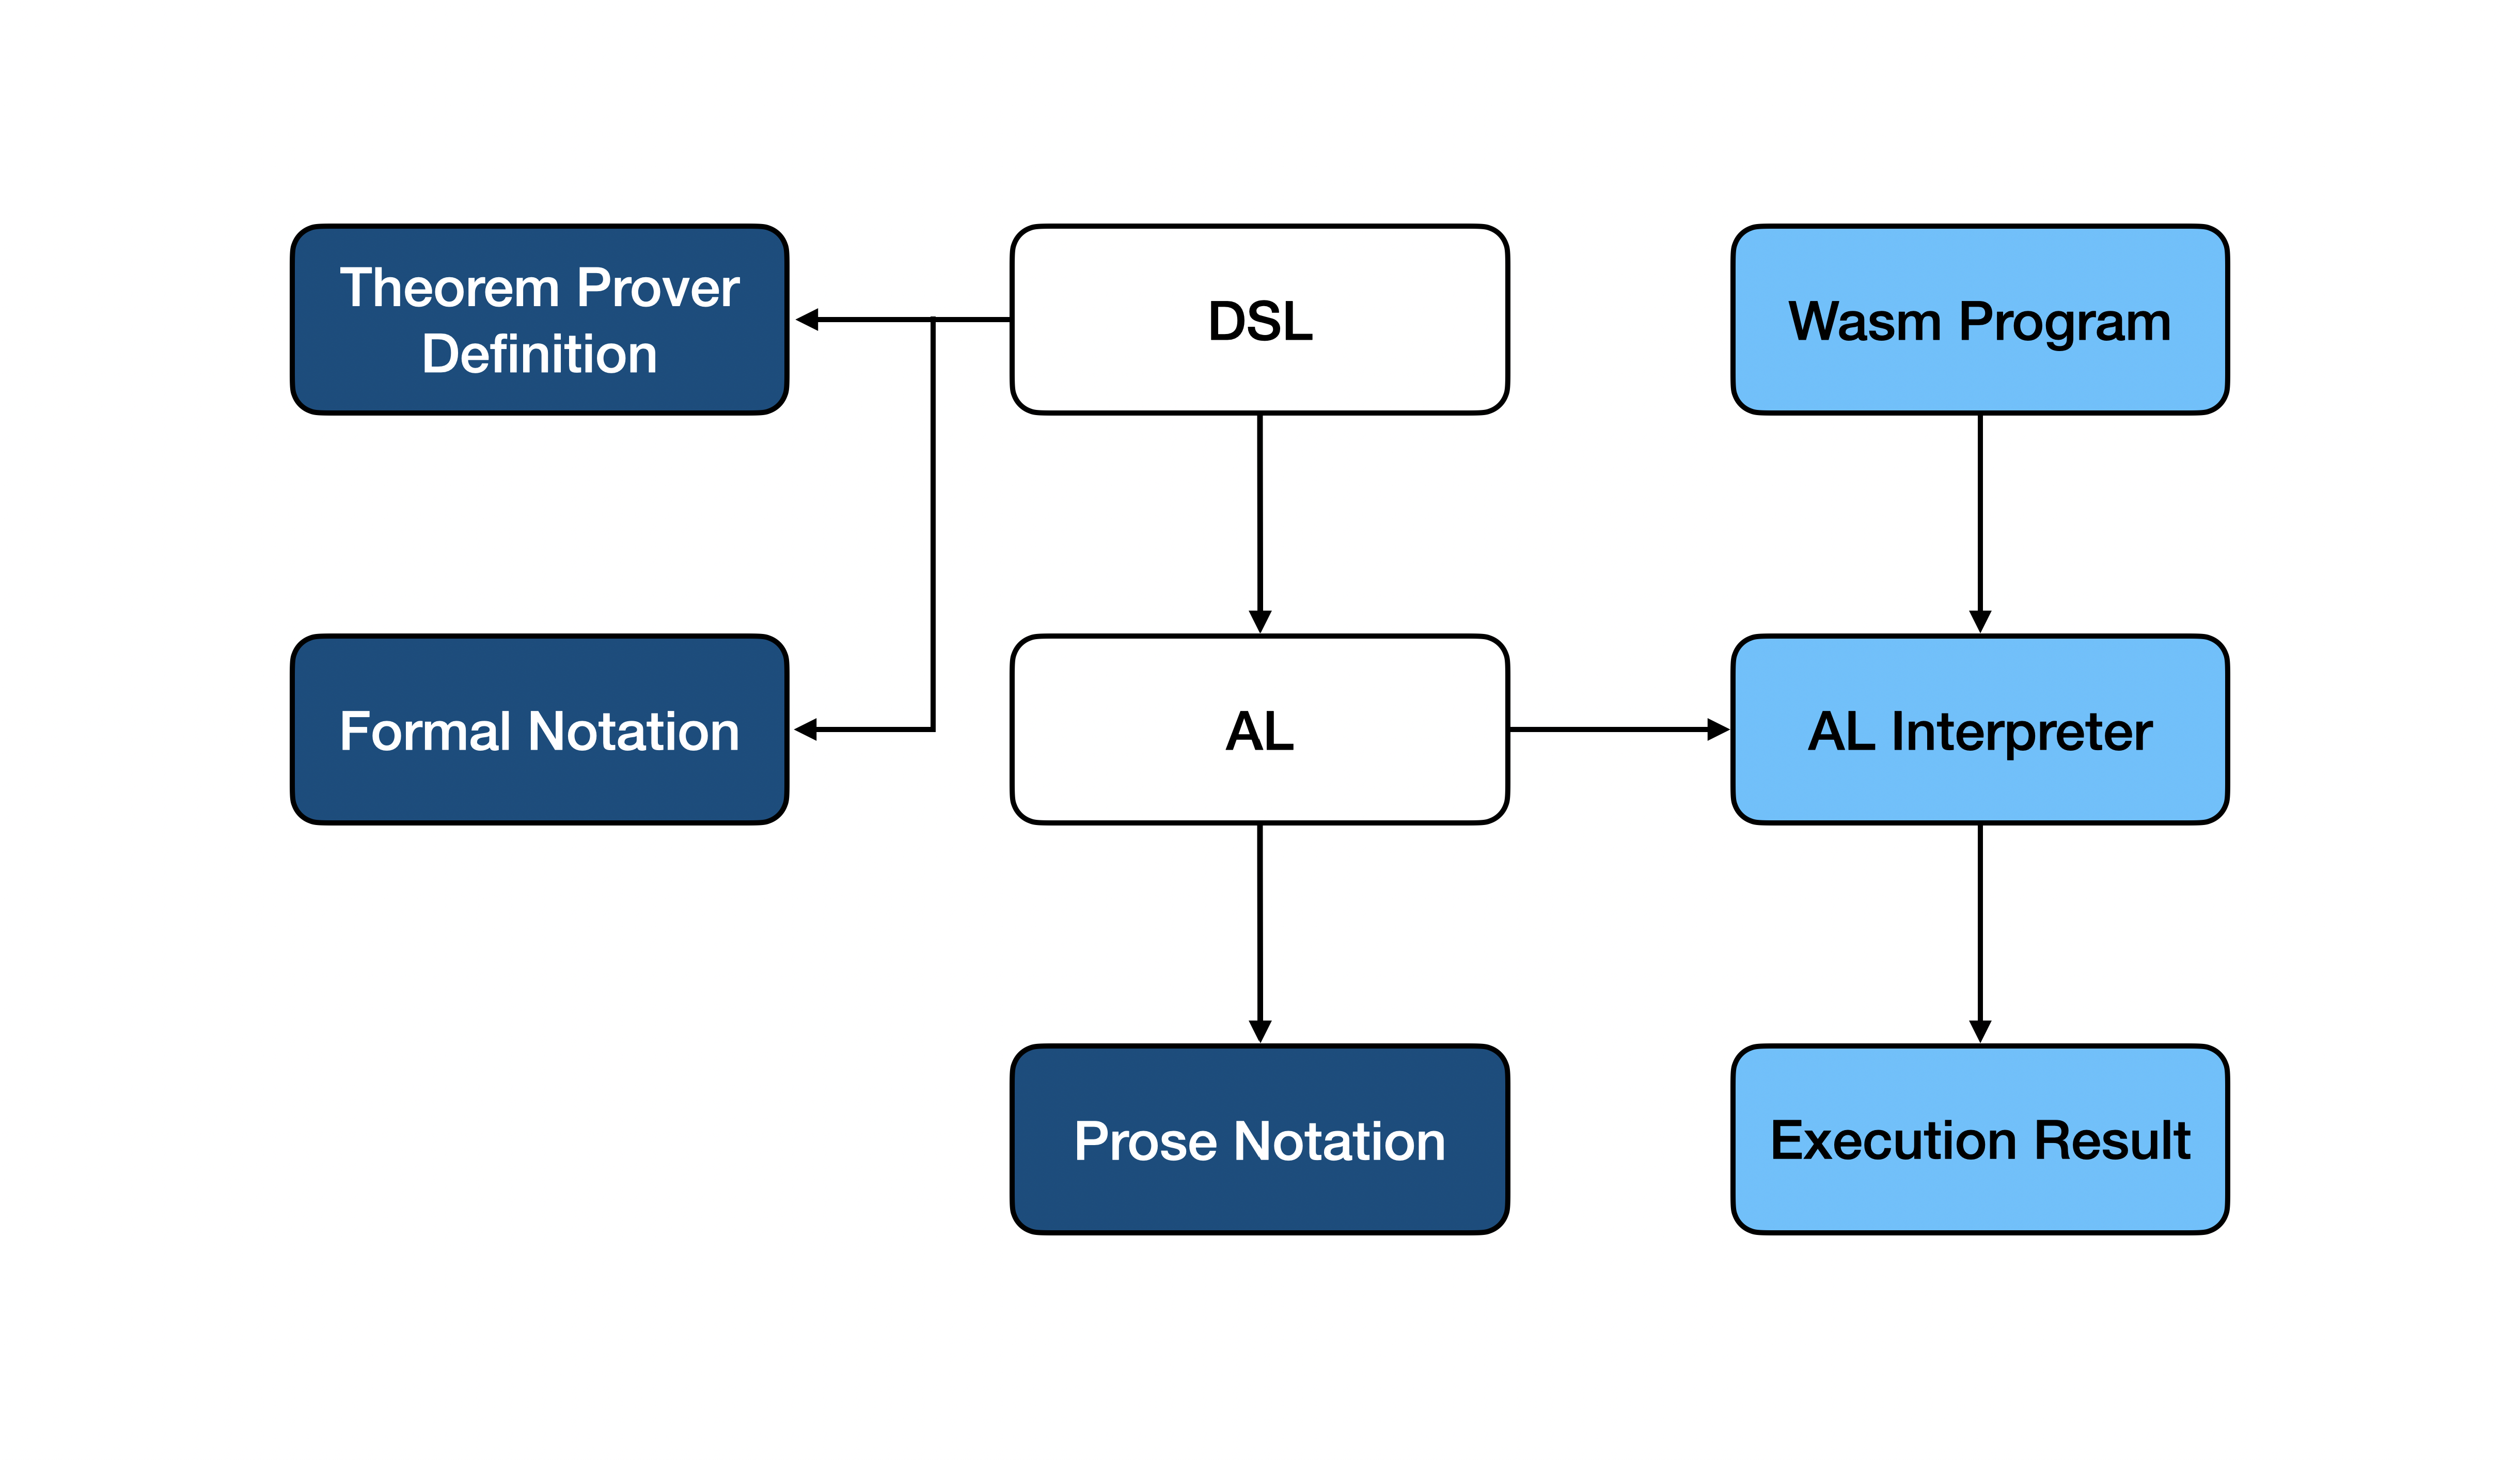
\includegraphics[width=15cm]{fig/overview}}
  \caption[An overview of the SpecTec architecture]
    {An overview of the SpecTec architecture}
    \label{fig:overview}
\end{figure}

% SpecTec: specification mechanization tool
SpecTec is a tool for \textit{mechanizing} WebAssembly specification
~\cite{spectec}.
Specification mechanization is a technique that treats a specification as data
that can be manipulated by a machine to automatically generate parser and
interpreter ~\cite{jiset}, to generate tests and perform differential tests
~\cite{jest}, to find meta-level errors in the specification ~\cite{jstar}, and
to perform meta-level static analysis for the static analysis of the defined
language ~\cite{jsaver}.
% Overview explanation
In this chapter, we explain the overall approach to generating multiple
artifacts from the specification and ensuring the correctness of the
specification.
\Cref{fig:overview} illustrates an overview of our approach.


% DSL
SpecTec offers a domain specific language (DSL) designed for writing
Wasm specifications.
It is a declarative language, providing a compact and user-friendly syntax.
This DSL can represent Wasm semantics in a manner closely resembling the formal
notation as shown in the following code for specification of testop
instruction.
The code below shows the specification for the \texttt{testop} instruction
written in the DSL:
\begin{lstlisting}[style=dsl]
rule Step_pure/testop:
(CONST nt c_1) (TESTOP nt testop)  ~>  (CONST I32 c)
-- if c = @\dollarcode@testop_(nt, testop, c_1)
\end{lstlisting}
The DSL is type checked to prevent meta-level errors such as notation misuses and
dimension mismatches.
Using the DSL, SpecTec generates LaTeX code and mechanized definitions for theorem provers.


% AL
Additionally, SpecTec introduces another imperative language, \textit{AL}, for
the prose notation.
In AL, semantics are expressed algorithmically, in the form of step-by-step
instructions that take inputs and perform operations, mirroring the prose notation.
SpecTec translates declarative definitions in the DSL into algorithmic
definitions in AL.
The AL code below is the specification for the \texttt{testop} instruction
generated from the DSL:
\begin{lstlisting}[style=al]
@\textbf{Step\_pure/testop}@ nt testop {
    Assert (check_type_of_stack_top(nt))
    Pop (CONST nt c_1)
    Let c = @$\dollarcode$@testop_(nt, testop, c_1)
    Push (CONST I32 c)
}
\end{lstlisting}
Using AL, SpecTec generates reStructuredText code.
\cref{fig:spectec-testop} shows the generated document for \texttt{testop}
instruction.
The generated document closely resembles the official document except for some
minor notation changes and some missing hyperlinks.


% AL interpreter
A notable feature of AL is that it is interpretable.
SpecTec includes an AL interpreter that executes an AL program with given inputs
and produces results.
Since an AL program specify the behavior of a Wasm program, the input to an AL
program is a Wasm program, and the result is the execution outcome of the Wasm
program.
In other words, the generated AL program functions as a WebAssembly interpreter.
What is particularly intriguing is that if specification authors write a Wasm
specification using the DSL, a WebAssembly interpreter that adheres to the
defined semantics is automatically generated.
By testing this generated interpreter, we can assess the specification,
thereby ensuring its correctness.
